\documentclass[a4paper]{article}

\usepackage[english]{babel}
\usepackage[utf8]{inputenc}
\usepackage{amsmath}
\usepackage{graphicx}
\usepackage{minted}
\usepackage{algorithm}
\usepackage[noend]{algpseudocode}
\usepackage[colorinlistoftodos]{todonotes}
\usepackage{multirow}
\usepackage{parskip}
\usepackage{tikz}


% empty set package
\usepackage{amssymb}

\title{ELEC 996 Bayesian Networks - Homework 4}
\author{Tian Gao}
\begin{document}
\maketitle

% Question 1
1. \\
There is an equivalent sample size N and $N = a_{11} + b_{11} = 12$ \\
Then each node should be checked.
$N_{31}=a_{31}+b_{31}=2$\\
$P(pa_{31}) * N = P(x_1=1,x_2=1) * N = P(x_1=1) * P(x_2=1) * N = \frac{4}{12} * \frac{6}{12} * 12=2=N_{31}$\\
$N_{32}=a_{32}+b_{32}=2$\\
$P(pa_{32}) * N = P(x_1=1,x_2=2) * N = P(x_1=1) * P(x_2=2) * N = \frac{4}{12} * \frac{6}{12} * 12=2=N_{32}$\\
$N_{33}=a_{33}+b_{33}=4$\\
$P(pa_{33}) * N = P(x_1=2,x_2=1) * N = P(x_1=2) * P(x_2=1) * N = \frac{8}{12} * \frac{6}{12} * 12=4=N_{33}$\\
$N_{34}=a_{34}+b_{34}=4$\\
$P(pa_{34}) * N = P(x_1=2,x_2=2) * N = P(x_1=2) * P(x_2=2) * N = \frac{8}{12} * \frac{6}{12} * 12=4=N_{34}$\\
So N=12 is the equivalent sample size.\\

% Question 2
2. \\
The augmented Bayesian network is shown as follows.\\
$a_{ij}=b_{ij}=\frac{N}{2q_i}$\\ 
$q_1=1, q_2=1, q_3=4, q_4=2$\\
(1) When N = 1\\
$a_{11}=b_{11}=0.5$\\ 
$a_{21}=b_{21}=0.5$\\
$a_{31}=b_{31}=0.125$\\
$a_{32}=b_{32}=0.125$\\
$a_{33}=b_{33}=0.125$\\
$a_{34}=b_{34}=0.125$\\
$a_{41}=b_{41}=0.25$\\
$a_{42}=b_{42}=0.25$\\

(2) When N = 2\\
$a_{11}=b_{11}=1$\\ 
$a_{21}=b_{21}=1$\\
$a_{31}=b_{31}=0.25$\\
$a_{32}=b_{32}=0.25$\\
$a_{33}=b_{33}=0.25$\\
$a_{34}=b_{34}=0.25$\\
$a_{41}=b_{41}=0.5$\\
$a_{42}=b_{42}=0.5$\\

(3) When N = 4\\
$a_{11}=b_{11}=2$\\ 
$a_{21}=b_{21}=2$\\
$a_{31}=b_{31}=0.5$\\
$a_{32}=b_{32}=0.5$\\
$a_{33}=b_{33}=0.5$\\
$a_{34}=b_{34}=0.5$\\
$a_{41}=b_{41}=1$\\
$a_{42}=b_{42}=1$\\

(4) When N = 10\\
$a_{11}=b_{11}=5$\\ 
$a_{21}=b_{21}=5$\\
$a_{31}=b_{31}=1.25$\\
$a_{32}=b_{32}=1.25$\\
$a_{33}=b_{33}=1.25$\\
$a_{34}=b_{34}=1.25$\\
$a_{41}=b_{41}=2.5$\\
$a_{42}=b_{42}=2.5$\\

\begin{figure}
\centering
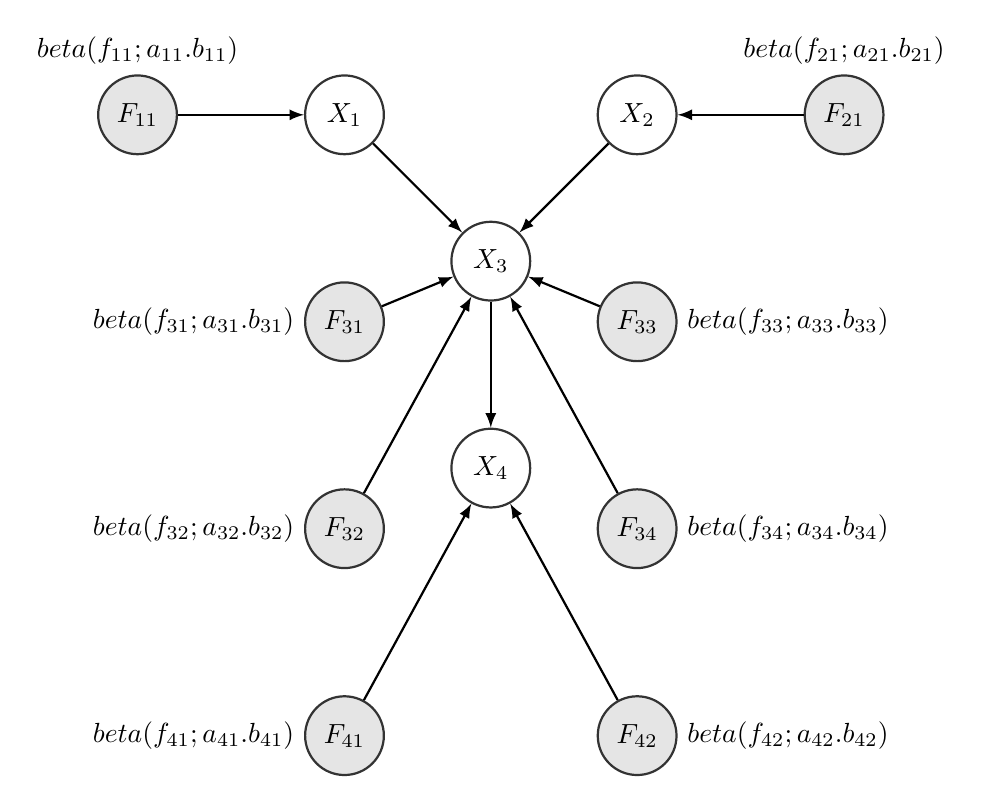
\begin{tikzpicture}
\tikzstyle{main}=[circle, minimum size = 10mm, thick, draw =black!80, node distance = 16mm]
\tikzstyle{connect}=[-latex, thick]
\tikzstyle{box}=[rectangle, draw=black!100]
  \node[main, fill = black!10] (f11) [label=above:$beta(f_{11};a_{11}.b_{11})$] {$F_{11}$};
  \node[main] (x1) [right=of f11] {$X_1$};
  \node[main] (x3) [below right=of x1] {$X_3$};
  \node[main] (x2) [above right=of x3] {$X_2$};
  \node[main, fill = black!10] (f21) [right =of x2, label=above:$beta(f_{21};a_{21}.b_{21})$] {$F_{21}$};
  \node[main, fill = black!10] (f31) [below=of x1, label=left:$beta(f_{31};a_{31}.b_{31})$] {$F_{31}$};
  \node[main, fill = black!10] (f32) [below=of f31, label=left:$beta(f_{32};a_{32}.b_{32})$] {$F_{32}$};
  \node[main, fill = black!10] (f33) [below =of x2, label=right:$beta(f_{33};a_{33}.b_{33})$] {$F_{33}$};
  \node[main, fill = black!10] (f34) [below =of f33, label=right:$beta(f_{34};a_{34}.b_{34})$] {$F_{34}$};
  \node[main] (x4) [below=of x3] {$X_4$};
  \node[main, fill = black!10] (f41) [below=of f32, label=left:$beta(f_{41};a_{41}.b_{41})$] {$F_{41}$};
  \node[main, fill = black!10] (f42) [below=of f34, label=right:$beta(f_{42};a_{42}.b_{42})$] {$F_{42}$};
  \path (f11) edge [connect] (x1)
  		(f21) edge [connect] (x2)
		(x1) edge [connect] (x3)
        (f31) edge [connect] (x3)
        (f32) edge [connect] (x3)
        (f33) edge [connect] (x3)
        (f34) edge [connect] (x3)
        (x2) edge [connect] (x3)
        (x3) edge [connect] (x4)
        (f41) edge [connect] (x4)
        (f42) edge [connect] (x4)        
        ;
\end{tikzpicture}
\end{figure}

% Question 3
3. \\
According to Theorem 6.14, \\
$a_{ij}=P(X_i=1|pa_{ij})*P(pa_{ij})*N$\\
$b_{ij}=P(X_i=2|pa_{ij})*P(pa_{ij})*N$\\
So:\\
$P(pa_{11}) = 1, a_{11}=\frac{3}{4}*36=27, b_{11}=\frac{1}{4}*36=9$\\
$P(pa_{21}) = 1, a_{21}=\frac{1}{3}*36=12, b_{21}=\frac{2}{3}*36=24$\\
$P(pa_{31}) = P(x_1=1)P(x_2=1)=\frac{1}{4}, a_{31}=\frac{1}{9}*\frac{1}{4}*36=1, b_{31}=\frac{8}{9}*\frac{1}{4}*36=8$\\
$P(pa_{32}) = P(x_1=1)P(x_2=2)=\frac{1}{2}, a_{32}=\frac{1}{2}*\frac{1}{2}*36=9, b_{32}=\frac{1}{2}*\frac{1}{2}*36=9$\\
$P(pa_{33}) = P(x_1=2)P(x_2=1)=\frac{1}{12}, a_{33}=\frac{1}{3}*\frac{1}{12}*36=1, b_{33}=\frac{2}{3}*\frac{1}{12}*36=2$\\
$P(pa_{34}) = P(x_1=2)P(x_2=2)=\frac{1}{6}, a_{34}=\frac{1}{6}*\frac{1}{6}*36=1, b_{34}=\frac{5}{6}*\frac{1}{6}*36=5$\\
$P(pa_{41}) = P(x_3=1) = \sum\limits_{i,j} P(x_3=1|x_1=i,x_2=j)P(x_1=i)P(x_2=j)=\frac{1}{3}$\\
$a_{41}=\frac{2}{3}*\frac{1}{3}*36=8, b_{41}=\frac{1}{3}*\frac{1}{3}*36=4$\\
$P(pa_{42}) = P(x_3=2) = \sum\limits_{i,j} P(x_3=2|x_1=i,x_2=j)P(x_1=i)P(x_2=j)=\frac{2}{3}$\\
$a_{42}=\frac{5}{8}*\frac{2}{3}*36=15, b_{42}=\frac{3}{8}*\frac{2}{3}*36=9$\\

\begin{figure}
\centering
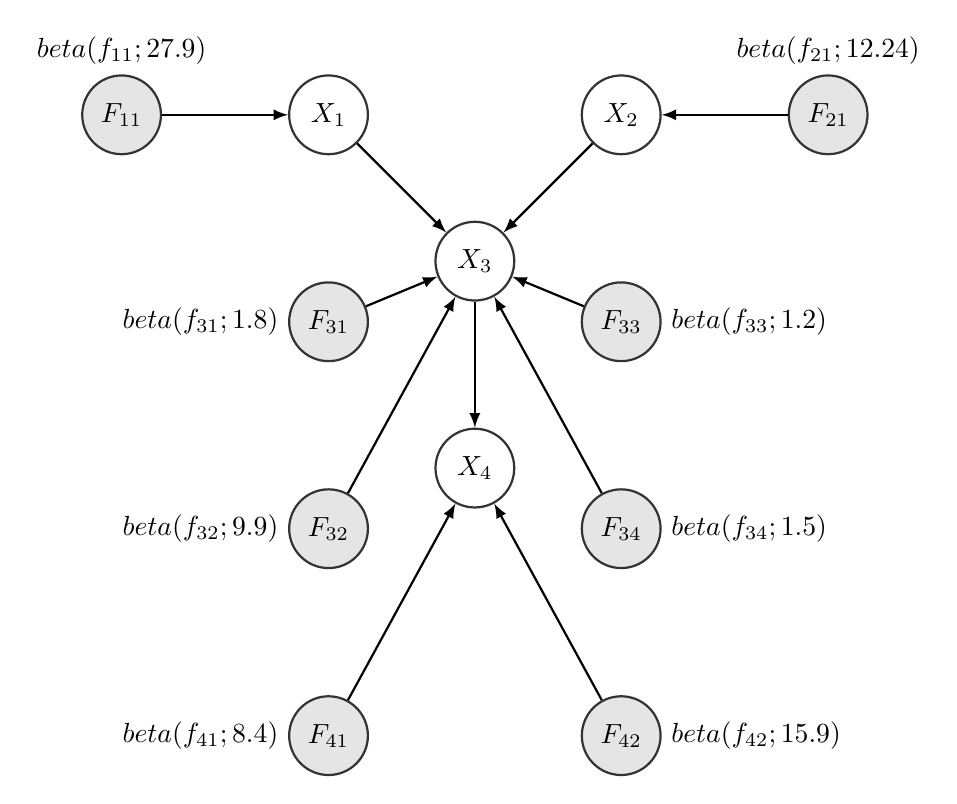
\begin{tikzpicture}
\tikzstyle{main}=[circle, minimum size = 10mm, thick, draw =black!80, node distance = 16mm]
\tikzstyle{connect}=[-latex, thick]
\tikzstyle{box}=[rectangle, draw=black!100]
  \node[main, fill = black!10] (f11) [label=above:$beta(f_{11};27.9)$] {$F_{11}$};
  \node[main] (x1) [right=of f11] {$X_1$};
  \node[main] (x3) [below right=of x1] {$X_3$};
  \node[main] (x2) [above right=of x3] {$X_2$};
  \node[main, fill = black!10] (f21) [right =of x2, label=above:$beta(f_{21};12.24)$] {$F_{21}$};
  \node[main, fill = black!10] (f31) [below=of x1, label=left:$beta(f_{31};1.8)$] {$F_{31}$};
  \node[main, fill = black!10] (f32) [below=of f31, label=left:$beta(f_{32};9.9)$] {$F_{32}$};
  \node[main, fill = black!10] (f33) [below =of x2, label=right:$beta(f_{33};1.2)$] {$F_{33}$};
  \node[main, fill = black!10] (f34) [below =of f33, label=right:$beta(f_{34};1.5)$] {$F_{34}$};
  \node[main] (x4) [below=of x3] {$X_4$};
  \node[main, fill = black!10] (f41) [below=of f32, label=left:$beta(f_{41};8.4)$] {$F_{41}$};
  \node[main, fill = black!10] (f42) [below=of f34, label=right:$beta(f_{42};15.9)$] {$F_{42}$};
  \path (f11) edge [connect] (x1)
  		(f21) edge [connect] (x2)
		(x1) edge [connect] (x3)
        (f31) edge [connect] (x3)
        (f32) edge [connect] (x3)
        (f33) edge [connect] (x3)
        (f34) edge [connect] (x3)
        (x2) edge [connect] (x3)
        (x3) edge [connect] (x4)
        (f41) edge [connect] (x4)
        (f42) edge [connect] (x4)        
        ;
\end{tikzpicture}
\end{figure}

% Question 4
4. \\
Assume $a_1$=5 means blood pressure is $<=$ 100\\
$a_2$=8 means blood pressure is 101-120\\
$a_3$=12 means blood pressure is 121-140\\
$a_4$=25 means blood pressure is 141-160\\
$a_5$=50 means blood pressure is $>=$ 161\\
So Dirichlet density function is Dir($f_1,f_2,f_3,f_4;5,8,12,25,50$)\\
P(blood pressure is $<=$ 100) $= \frac{5}{100}=0.05$\\
P(blood pressure is 101-120)$ = \frac{8}{100}=0.08$\\
P(blood pressure is 121-140)$ = \frac{12}{100}=0.12$\\
P(blood pressure is 141-160)$ = \frac{25}{100}=0.25$\\
P(blood pressure is $>=$ 16)$ = \frac{50}{100}=0.5$\\

% Question 5
5. \\
Since $a_1=5, a_2=8, a_3=12, a_4=25, a_5=50, N=100$\\
And $s_1=2, s_2=15, s_3=23, s_4=25, s_5=35, M=70$\\
(1) $P(d)=\frac{\Gamma(100)}{\Gamma(170)}\frac{\Gamma(7)}{\Gamma(5)}\frac{\Gamma(23)}{\Gamma(8)}\frac{\Gamma(35)}{\Gamma(12)}\frac{\Gamma(50)}{\Gamma(25)}\frac{\Gamma(85)}{\Gamma(50)}$\\
(2)$\rho(f|d)=Dir(f_1, f_2, f_3, f_4;7, 23, 35, 50, 85)$\\
(3)$P(x^{M+1}=k|d)=\frac{a_k+s_k}{M+N}$\\
So $P(x^{M+1}is <= 100|d)=\frac{7}{170}$\\
$P(x^{M+1}is 101-120|d)=\frac{23}{170}$\\
$P(x^{M+1}is 121-140|d)=\frac{35}{170}$\\
$P(x^{M+1}is 141-160|d)=\frac{50}{170}$\\
$P(x^{M+1}is >= 161|d)=\frac{85}{170}$\\

% Question 6
6. \\
a.\\
$a_{111}=4, s_{111}=5, a_{112}=8, s_{112}=6, a_{113}=10, s_{113}=4, N_{11}=22, M_{11}=15$\\
$a_{211}=1, s_{211}=2, a_{212}=1, s_{212}=1, a_{213}=1, s_{213}=1, a_{214}=1, s_{213}=1, N_{21}=4, M_{21}=5$\\
$a_{311}=2, s_{311}=3, a_{312}=4, s_{312}=2, a_{313}=1, s_{313}=1, a_{314}=1, s_{313}=0, N_{31}=8, M_{31}=6$\\
$a_{411}=1, s_{411}=0, a_{412}=3, s_{412}=1, a_{413}=4, s_{413}=1, a_{414}=2, s_{413}=2, N_{41}=10, M_{41}=4$\\
So $P(d)=\prod\limits_{i=1}^{n} \prod\limits_{j=1}^{q_i} \frac{\Gamma(N_{ij})}{\Gamma(N_{ij}+M_{ij})} \prod\limits_{k=1}^{r_i} \frac{\Gamma(a_{ijk}+s_{ijk})}{\Gamma(a_{ijk})}=\frac{\Gamma(22)}{\Gamma(37)}\frac{\Gamma(9)}{\Gamma(4)}\frac{\Gamma(14)}{\Gamma(8)}\frac{\Gamma(14)}{\Gamma(10)} \times \frac{\Gamma(4)}{\Gamma(9)}\frac{\Gamma(3)}{\Gamma(1)}\frac{\Gamma(2)}{\Gamma(1)}\frac{\Gamma(2)}{\Gamma(1)}\frac{\Gamma(2)}{\Gamma(1)} \times \frac{\Gamma(8)}{\Gamma(14)}\frac{\Gamma(5)}{\Gamma(2)}\frac{\Gamma(8)}{\Gamma(4)}\frac{\Gamma(6)}{\Gamma(1)}\frac{\Gamma(1)}{\Gamma(1)} \times \frac{\Gamma(10)}{\Gamma(14)}\frac{\Gamma(1)}{\Gamma(1)}\frac{\Gamma(4)}{\Gamma(3)}\frac{\Gamma(5)}{\Gamma(4)}\frac{\Gamma(4)}{\Gamma(2)}$\\

b.\\
\begin{figure}[htb]
\centering
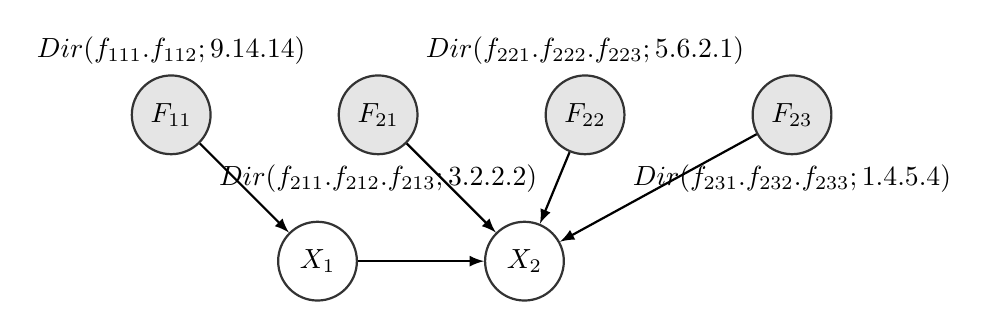
\begin{tikzpicture}
\tikzstyle{main}=[circle, minimum size = 10mm, thick, draw =black!80, node distance = 16mm]
\tikzstyle{connect}=[-latex, thick]
\tikzstyle{box}=[rectangle, draw=black!100]
  \node[main, fill = black!10] (f11) [label=above:$Dir(f_{111}.f_{112};9.14.14)$] {$F_{11}$};
  \node[main] (x1) [below right=of f11] {$X_1$};
  \node[main] (x2) [right=of x1] {$X_2$};
  \node[main, fill = black!10] (f21) [right =of f11, label=below:$Dir(f_{211}.f_{212}.f_{213};3.2.2.2)$] {$F_{21}$};
  \node[main, fill = black!10] (f22) [right =of f21, label=above:$Dir(f_{221}.f_{222}.f_{223};5.6.2.1)$]{$F_{22}$};
  \node[main, fill = black!10] (f23) [right =of f22, label=below:$Dir(f_{231}.f_{232}.f_{233};1.4.5.4)$]{$F_{23}$};
  \path (f11) edge [connect] (x1)
		(x1) edge [connect] (x2)
        (f21) edge [connect] (x2)
        (f22) edge [connect] (x2)
        (f23) edge [connect] (x2)
        ;
\end{tikzpicture}
\end{figure}

c.\\
$P(x_1=1)=\frac{9}{37}$\\
$P(x_1=2)=\frac{14}{37}$\\
$P(x_1=3)=\frac{14}{37}$\\

$P(x_1=1|x_1=1)=\frac{1}{3}$\\
$P(x_1=2|x_1=1)=\frac{2}{9}$\\
$P(x_1=3|x_1=1)=\frac{2}{9}$\\
$P(x_1=4|x_1=1)=\frac{2}{9}$\\

$P(x_1=1|x_1=2)=\frac{5}{14}$\\
$P(x_1=2|x_1=2)=\frac{3}{7}$\\
$P(x_1=3|x_1=2)=\frac{1}{7}$\\
$P(x_1=4|x_1=2)=\frac{1}{14}$\\

$P(x_1=1|x_1=3)=\frac{1}{14}$\\
$P(x_1=2|x_1=3)=\frac{2}{7}$\\
$P(x_1=3|x_1=3)=\frac{5}{14}$\\
$P(x_1=4|x_1=3)=\frac{2}{7}$\\

d.\\
$P(x_1=3,x_2=4)=P(x_2=4|x_1=3)P(x_1=3)=\frac{4}{37}$\\

e.\\
$P(x_1=3)=\sum\limits_{i}P(x_2=i|x_1=3)P(x_1=3)=\frac{14}{37}$\\

\end{document}
